\clearpage
%%----------------------------------------------------------------------
%%----------------------------------------------------------------------
\missiontitle{Mission: Skirmish}

\begin{columns}

\bigskip\missionheading{Summary}%

\smallskip\noindent Outriders patrolling the outskirts of their main
forces have crashed into each other---contact is made!  No quarter is
given as the hot flames of war leap to life.

\smallskip {\bf Campaign Play:} Attacker and Defender roles are
identical in this mission and have no effect in-game.

\bigskip\missionheading{The Battlefield}%

\smallskip\noindent The mission is played on a~4'x4' table.  A variety
of ruins, woods, and other terrain should cover a quarter to a half of
the board, roughly symmetrically.

Deployment zones are diagonal table corners, up to~12'' from the
centerline between them.  Roll off to determine who chooses a corner
and their player table edge, the other player taking the opposite.

Objective markers are placed at the center of the table and the
centers of the two table quadrants opposite the deployment zone
corners.

\bigskip\missionheading{Mission Rules}%

Roll off to determine who decides which player deploys first.  After
both players deploy, the player that setup first chooses to play first
or second.  The player to go second may attempt to Seize the
Initiative.

Night Fighting is in effect for Turn~1 on a~D6 of~4+; on a~1 or~2 it
takes effect on Turn~5 and thereafter.

The Variable Game Length rule applies.  At game end use the scoring
chart to determine the victor!

%\vfill
%\vbox to 0pt {}

\columnbreak

\noindent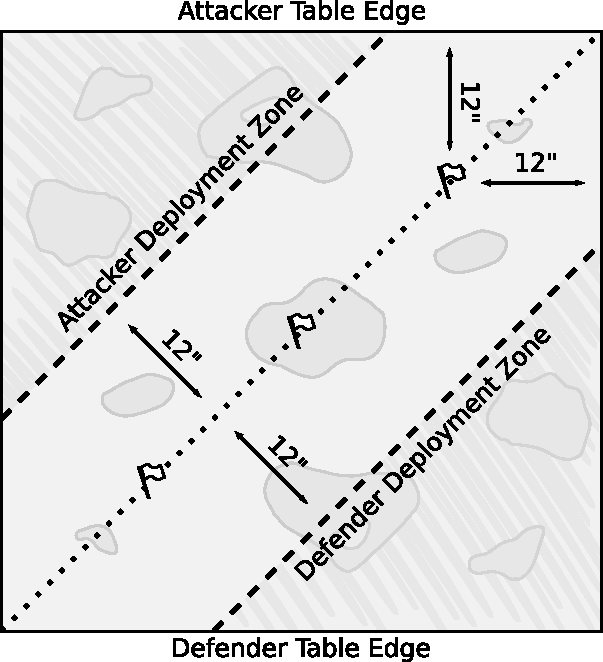
\includegraphics[width=\linewidth]{maps/skirmish.pdf}

\vspace*{12pt}

\noindent\vbox{%
\noindent\vbox to -4pt{\noindent\hfill\Large\bf\sc\fontfamily{ptm}\selectfont Scoring\vbox{}}\\
%
\noindent\fbox{\vbox{\small%
\setlength{\tabcolsep}{2pt}%
\noindent\begin{tabularx}{\linewidth}{cccX}
  \hbox to 1.25em{\rotatebox{45}{\small\bf Attacker}}&
  \hbox to 1.25em{\rotatebox{45}{\small\bf Defender}}&
  &
  \multicolumn{1}{c}{\footnotesize\bf Condition}
\\
  \hline
%
  \rescheck&\rescheck& & {\bf Major Victory:} Player controls at least
  two more objective markers than opponent, or opponent has been
  completely eliminated.\\
%
  \rescheck&\rescheck& &
  {\bf Minor Victory:} Player controls at least one more
                       objective marker than opponent.\\
%
\rescheck&\rescheck& &
{\bf Draw:} Players control equal objective markers.\\
\hline \rescheck&\rescheck& &
{\bf Bonus Point:} Opponent's leader is not on table.\\
\rescheck&\rescheck& &
{\bf Bonus Point:} Player has at least one model within 12'' of each table corner.\\
\end{tabularx}%
}}}

\end{columns}
